% Nejprve uvedeme tridu dokumentu s volbami
\documentclass[bc,female,java,dept456]{diploma}						% jednostranny dokument
\usepackage[czech]{babel}
%\usepackage[cp1250]{inputenc}
\usepackage[utf8]{inputenc}
\usepackage{comment}
\usepackage{graphicx}
\usepackage{url}
%\usepackage{dialogue}

\setcounter{secnumdepth}{2}


\begin{comment}
> Zdravím, tak jsem to proletěl.
>
> - co citování zdrojů? Např. v části o učňovství atd,. to určitě není z Vaší hlavy
> - moc se mi nezdá vyvážení textu, moc stránek věnujete existujícím nástrojům
> - používejte méně osobní formy zápisu, jako udělám, mám, chci atd. kspíše obecně a neosobně, co je v práci obsaženo. Když napíšte, chci navrhnout rozhraní, tak to vypadá blbě, protože pro úspěšné zvládnutí diplomky jste ho snad už navrhnul a realizoval
> - v kapitole 5 není moc jasné vazba mezi prezentovanými informacemi ani to jestli je to Vaše práce nebo ne. Zdůrazněte, co je výstupem diplomky a proč
> - více referencí
> - druhá část mi příjde zmatená a bez nosných informací, ale možná, že to ještě nemáte hotovo.
\end{comment}



% Zadame pozadovane vstupy pro generovani titulnich stran.
\Author{Michal Hantl}

\Title{Nástroj pro monitorování chování uživatelů webových aplikací}

\EnglishTitle{A tool for monitoring web application user behaviour}

\SubmissionDate{20. dubna 2011}

\PrintPublicationAgreement{true}




\Thanks{Rád bych na tomto místě poděkoval svým rodičům za podporu během celého studia, panu Ing. Michalovi Radeckému, za vedení během vypracování diplomové práce a své přítelkyni Míše.}





\CzechAbstract{
Cílem práce je vytvoření nástroje, jakožto podpory pro aplikaci a navržení metody získávání informací o chování uživatele webové aplikace. Nebude se jednat o klasický přístup založený na sběru statistických dat anonymních návštěvníků, ale o využití znalosti o konkrétním uživateli, jeho chování, využívání funkcí a služeb webové aplikace.

Výsledkem praktické části je webová aplikace ...
}

\CzechKeywords{webová analytika, chování uživatelů, webová aplikace, diplomová práce}

\EnglishAbstract{
The goal of this thesis is to create a tool to aid web application development and to create a method for gaining knowledge of the web application users' behaviour. It is not the case of usual anonymized data gathering, but make us of the knowledge of concrete user, his behaviour and his usage of web app's functions and services. 
}

\EnglishKeywords{web analytics, user behaviour, web application, master thesis}





% Pridame pouzivane zkratky (pokud nejake pouzivame).
\AddAcronym{GUI}{Grafické uživatelské rozhraní (Graphical User Interface)}
\AddAcronym{HTML}{Jazyk pro vytváření webových stránek (HyperText Markup Language)}





% Zacatek dokumentu
\begin{document}

% Nechame vysazet titulni strany.
\MakeTitlePages

% Asi urcite budeme potrebovat obsah prace.
\tableofcontents
\cleardoublepage	% odstrankujeme, u jednostranneho dokumentu o jednu stranku, u oboustrenneho o dve

% Jsou v praci tabulky? Pokud ano vysazime jejich seznam.
% Pokud ne smazeme nasledujici makro.
%\listoftables
%\cleardoublepage	% odstrankujeme, u jednostranneho dokumentu o jednu stranku, u oboustrenneho o dve

% Jsou v praci obrazky? Pokud ano vysazime jejich seznam.
\listoffigures
\cleardoublepage	% odstrankujeme, u jednostranneho dokumentu o jednu stranku, u oboustrenneho o dve


% Jsou v praci vypisy programu? Pokud ano vysazime jejich seznam.
\lstlistoflistings
\cleardoublepage	% odstrankujeme, u jednostranneho dokumentu o jednu stranku, u oboustrenneho o dve






\section{Úvod (3 stránky)}
\label{sec:Uvod}


Tato diplomová práce se zabývá webovou analytikou. Úvodem popisuje jaký problém webová analytika řeší, nastiňuje historii měření na webu a současné nejčastější využití nástrojů pro webovou analytiku.

V první kapitole popisuje nejčastěji používané techniky měření a vizualizace dat, vysvětluje motivace za jednotlivými technikami a případy užití.

Druhá kapitola se zabývá návrhem nové techniky měření, která se zajímá o to, které funkce webové aplikace uživatelé používají. Popisuje jakým způsobem budou data získána a celý systém jako celek.

Třetí kapitola "Implementace" je zaměřena na použité tehcnologie a konkrétní procesy sběru a analýzy dat.

Čtvrtá kapitola následuje aplikací vzniklého nástroje na existující webovou aplikaci. Cílem je ověřit, že vyvinutý nástroj přináší očekávané výsledky.

V poslední kapitole dochází ke zhodnocení zda metoda měření i nástroj plní očekávání, jaký je jejich přínos pro jejich uživatele v praxi a porovnání s podobnými nástroji.


\subsection{Hostorie webové analytiky}

\subsubsection{1990 - Zrození WWW stránek}
Na začátku devadesátých let došlo ke zrození WWW stránek[reference]. Uživatelé tehdy prohlíželi statické stránky a pokaždé, když si nějakou prohlédli, vznikl záznam v logovacím souboru, takzvaný "hit". Počet hitů se stal ukazatelem úspěšnosti webový stránek.

\subsubsection{1994 - Mosaic: První masově úspěšný grafický prohlížeč}
V roce devadesát čtyři vznikl grafický webový prohlížeč s názvem Mosaic[reference]. Díky jeho snadné instalaci a srozumitelnému uživatelskému rozhraní se web otevřel široké veřejnosti. Tento prohlížeč byl později přejmenován na Netscape a v roce 1995 ho používalo 80\% uživatelů internetu.

\subsubsection{1995 - Analog: Analýza logovacích souborů}
V roce devadesát pět znikl Analog - nástroj pro analýzu logovacích souborů. Jeho autor Stephen Turner ho poskytoval zdarma jako freeware pro několik platform. Jednalo se o první sofistikovaný nástroj pro analýzu a zobrazení návštěvnosti webových stránek.

\begin{lstlisting}[label=src:Plain,caption=Ukázka záznamu z logovacího souboru ve formátu RFC931]
10.20.30.40 - - [26/Apr/2000:00:23:48 -0400] "GET /index.html HTTP/1.0" 200 6248 "http://www.jafsoft.com/asctortf/" "Mozilla/4.05 (Macintosh; I; PPC)"
10.20.30.40 - - [26/Apr/2000:00:23:48 -0400] "GET /background.gif HTTP/1.0" 200 4005 "http://www.example.org/" "Mozilla/4.05 (Macintosh; I; PPC)"
\end{lstlisting}

Logovací soubor obsahuje jden řádek pro každou návštěvu stránky, nebo souboru na serveru. Nástroj pro analýzu logovacích souborů z toho pak dokáže zjistit kolik měl server návštěv každý den, z kolika unikátních IP adres, které stránky jsou nejnavštěvovanější a kolik bylo přenesených dat.

The data collection became unusable with the advent of search engines and their robots, proxies servers to surf anonymously, allocation of dynamic IP addresses by ISPs and cached content techniques. All these developments have rendered the use of log files inappropriate to analyze user behavior. The data contained in log files were indeed biased and unique visitor identification almost impossible. 

\begin{figure}[h]
	\centering
	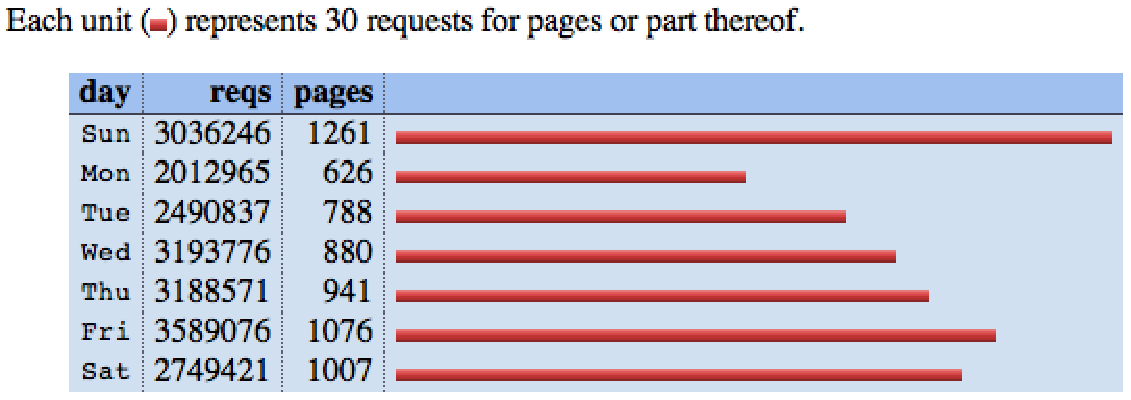
\includegraphics[width=14cm]{img/analog_daily.pdf}
	\caption{Analog - denní návštěvnost}
	\label{analog_daily}
\end{figure}


\subsubsection{1996 - Měření pomocí kódu na stránce}

V roce 1996 byl v obou nejpoužívanějších prohlížečích\footnote{V roce 1996 měl Netscape Navigator zhruba 80\% podíl a Internet Explorer 14\%} k dispozici JavaScript. 

Tvůrce webových stránek na každou stránku umístil kód, který mu vygeneroval poskytovatel měřícího nástroje. 


Tento postup se zásadně liší od analýzy logových souborů. Místo statické analýzy zaznamenaných dat na straně serveru tento přístup data dynamicky sbírá na straně klienta.

Tento průlom umožnil použtití třetích stran pro sběr i vyhodnocení dat a tak dal vzniknout prvním online nástrojům pro webovou analytiku. V různých obměnách se tato technika používá dodnes.


\subsubsection{2005 - Moderní webová analytika pro každého}

V roce 2005 koupila společnost Google analytický systém Urchin on Demand a ještě v témž roce ho poskytla zdarma široké veřejnosti jako webovou aplikaci pod názvem Google Aanlytics.

Pro obrovský zájem byl tento produkt zpřístupněn pouze omezenému počtu uživatelů. Od října roku 2006 byly znovu otevřeny volné registrace a dodnes se jedná o nejpoužívanější systém pro webovou analytiku.


\subsubsection{2011 - Sociální média a zařízení}

S nástupem sociálních médií a chytrých mobilních zařízení dochází k nárůstu času, který uživatelé tráví na internetu. Poměrně k tomuto nárůstu se zvyšují investice do internetových stránek a webových aplikací. 

Na jedné straně je snaha dostat nové uživatele na svou stránku, to se dociluje například pomocí optimalizace pro vyhledávače, reklamních bannerů, nebo PPC reklamy\footnote{PPC - Pay per click, platba se za proklik (cena prokliku je určena pomocí aukce).}. V tomto případě slouží webová analytika k měření efektivity jednotlivých kampaní a k jejich následné optimalizaci.

Na druhé je snaha pracovat s uživateli, které už webová stránka, nebo aplikace má. Zde je snaha identifikovat problémy a optimalizavat uživatelskou zkušenost. V obou případech je to webová analytika, která nám umožňuje získat přehled, optimalzovat a vyhodnotit návratnost investic.




\section{Sběr a interpretace dat (15 stránek)}

Podstatou webové analytiky je sběr a interpretace dat. Jak již bylo řečeno, sběr dat se za dobu existence webu vyvinul z pasivní formy analýzy logových souborů na serveru do dnešní - aktivního sběru dat na straně uživatele třetí stranou.

Tato kapitola popisuje jak sběr dat, tak jejich interpretaci.

\subsection{Analýza dat z logovacích souborů}

\subsection{Události v prohlížeči}

\subsubsection{Pohyb myši}
\subsubsection{Klikání}
\subsubsection{Používání kláves}
\subsubsection{Odchod ze stránky}
\subsubsection{Skrolování stránky}
  
\subsection{Informace získané pomocí HTTP protokolu}
\subsubsection{Prohlížeč a verze}
\subsubsection{Geolokace}
\subsubsection{referrer}
\subsubsection{stránka}
\subsubsection{query string}

\subsection{Informace získané pomocí JavaScriptu}
\subsubsection{Rozlišení obrazovky}
\subsubsection{Velikost viewportu}
(zobrazení stránek, jako analýza logů)
 

\subsection{Derivované informace}
\subsubsection{Doba strávená na stránce}
\subsubsection{Loajalita = opakování návštěv}
\subsubsection{Častost návštěv}
\subsubsection{Počet návštěv}
\subsubsection{Počet unikátních uživatelů}
  
  

\subsection{Interpretace a Vizualizace dat}

\subsubsection{Heatmapy}
\subsubsection{Heatmapy}
\subsubsection{Světová mapa}
\subsubsection{Segmentace}


Aplikace v praxi
 - optimalizace kampaní
 - A/B / split testing




\subsection{Clickstream analýza}

\subsection{Měření konverze}






\section{Návrh (15 stránek s diagramy)}

O čem je tahle kampitola?

\subsection{Hypotéza}

Popis problému.

Demonstrovat na příkladu.

Popis řešení.

Co se bude měřit a proč.

Co nástroj dělá a proč.

Co nástroj nedělá a proč ne.

Pro koho je nástroj určen.

Existuje nějaký podobný nástroj?

Proč takový nástroj ještě neexistuje?
(implementujou si in house řešení tohoto problému)

\subsection{Sběr dat}

Jaké data nás zajímají a proč

Jaké data nás nezajímají a proč

Jaké jsou omezení sběru dat.


\subsection{Interpretace dat}

Jaké možnosti interpretace dat jsou?

Jaké možnosti se hodí?

Jaké možnosti intepretace dat jsme zvolili a proč?

Jaké jsou možnosi segmentace. 
Jaké jsou možnosti do budoucna.

Možnosti aproximace?


\subsection{Etická stránka sběru dat}

Problém etiky sběru dat.
Právní problémy.
Anonymní vs. neanonymní data.
Webaplikace vs. webová stránka.
Zákazník vs. náhodný návštěvník.
Analogie z fyzického byznysu.





\section{Implementace (20 stránek i s grafy)}

O čem je tato kapitola?


\subsection{Popis technického řešení (10 Stran)}

1) diagram celého systému

2) detail sběru dat

3) detail interpretace dat

4) zobrazení dat


vizualizační technologie, appengine
proč jsem vybral tyto technologie
detaily funkce měřícího skriptu (AES)
detaily sběru dat
detaily analýzy dat



\subsection{Aplikace v reálném provozu (10 stran i s grafy)}

oběcně kolik dat tam lítalo denně, kolik uživatelů
analýza dat (na co jsem se zaměřil)
zajímavé grafy, co z nich vyplývá
závěry (navhrnout změny)

\subsection{Navrhnuté změny na základě získaných dat (2 stránky)}


\section{Zhodnocení (2 stránky)}
co splnilo očekávání
co nesplnilo / předčilo očekávání
přínos pro uživatele v praxi
porovnání s podobnými nástroji




\section{Závěr (1 stránka)}
\label{sec:Conclusion}

Byla to bomba :)

\bigskip
\begin{flushright}
Michal Hantl
\end{flushright}









\begin{thebibliography}{99}


\bibitem{peci2005} Pecinovský, Rudolf,
\textit{Jak efektivně učit OOP. Tvorba softwaru 2005 – sborník přednášek}, ISBN 80-86840-14-X.

\bibitem{peci_trendy} Pecinovský, Rudolf,
\textit{Současné trendy v metodice výuky programování}, dostupné z url \url{http://gynome.nmnm.cz/konference/files/2006/sbornik/pecinovsky.pdf}.

\bibitem{plaminek} Plamínek, Jiří,
\textit{Tajemství motivace – Jak zařídit, aby pro vás lidé rádi pracovali}, ISBN 80-247-1991-6.

\bibitem{kamarati} Gašparovičová Ľuba, Hvorecký, Josef,
\textit{Kamaráti Robota Karla}, ISBN 80-06-00421-8.

\end{thebibliography}


%\appendix
%\section{Grafy a měření}
%Tohle je příloha k práci. Většinou se sem dávají grafy, tabulky, které by vzhledem
%ke svému počtu překážely v textu diplomky.
%\clearpage




\end{document}